%---------------------------------------------------------------
\chapter{Beyond Pollution}
%---------------------------------------------------------------

\todo{actually name it}

\begin{chapterabstract}
	\todoadd
\end{chapterabstract}

After observing that the pollution happens in the compiler, the next step is to understand how the feedback slots infulence the compilation of a function. In order to do this, we need to categorize the slots.

\todo{why do we do it}

In this chapter, we only focus on the \textit{type slots}, because as previously observed these suffer from pollution the most and are the ones that are changing the most, providing a richer analysis.

The Ř compiler does \textit{optimistic speculations} on the feedback slots \todo{better wording}. This means that when a PIR instruction with an attached type feedback is observed, we emit an assumption on the type and the a cast to this type (a nop in the native code) in hopes that this unlocks some optimizations later. This has advantage that if an optimization is based on many complex speculations, it will be applied. The disadvanatge is that we might restrict the type more than is necesarry, e.g. we might speculate on a more specific type than is needed.

This is contrary to how most other JIT compiler do speculations, like the JavaScript V8 VM\todocite, where they only emit an assumption on a type at the point where the type is used.

%---------------------------------------------------------------
\section{Definitions}
%---------------------------------------------------------------

First, we separate the \textit{empty} and \textit{non-empty} slots. The empty slots are not interesting, as they are paths of the program that are not excercised.

We say that a slot is \textit{referenced} if it is part of a function that is compiled to native, including slots inside of inlined functions. A slot is then \textit{read} if during this compilation the information in the slot is observed. A \textit{used slot} is a type feedback slot that has an assumption connected with it in the final version of PIR (after all optimizations finished running). A used slot is always non-empty.

%---------------------------------------------------------------
\subsubsection*{Used slots}
%---------------------------------------------------------------

When an assumption on a type is emited, it has a structure outlined in listing \ref{lst:assume-structure}. The value we speculate on is in the register \texttt{\%1} with a \textit{static type}, which is inferred from the call context, known types of builtins, and preceding assumtions. The instruciton has also an associated \textit{feedback type}, which is the union of types observed in the interpreter. The speculated value is an input to an \texttt{IsType} instruction, which checks the actual runtime type against the \textit{assumed type}. The result of the type check is then an input to the \texttt{Assume} instruction, along with the corresponding \texttt{Checkpoint}. If the type check fails (\texttt{\%2} is false), we trigger a deoptimization and restore the frame state according to the checkpoint, otherwise we continue with execution.

\begin{listing}[H]
  \centering
	\begin{minted}[linenos=false]{\pirlexer}
<static type>   %1    = <instruction>       args... <feedback type>
lgl$#-          %2    = IsType              %1 isA <assumed type>
void                    Assume              %2, <checkpoint> (Typecheck[Type#N])
  \end{minted}
	\caption{PIR code structure of type assumption}\label{lst:assume-structure}
\end{listing}

The construction of the assumed type is not as straight-forward as it might seem (illustrated in figure \ref{fig:types-venn}). First, we construct an \textit{expected type} by intersecting the static and feedback type. If this intersection is empty, no assumption is emited and the feedback type is empty, otherwise we procede to create the assumed type.

\begin{figure}
	\centering
	\includediagram{8}
	\caption{Illustration of the relationship between static, feedback, expected and assumed types}\label{fig:types-venn}
\end{figure}

It can happen that the static type is more precise than the feedback type, and the feedback type is not a subtype of the expected type (in the figure \ref{fig:types-venn}, the green area is non-empty). We call this a \textit{narrowing} of the feedback type with the static type. For example, this happens when we statically know that the value we are speculating on is a scalar, but we have observed also non-scalar values.

If the R type of the expected type is not integer, float or logical vector, we do not speculate on it as it is. The optimizations are not able to use this precise of an information, thus the compiler tries to relax the assumption first. We call this \textit{widening}, as we are widening the information of the feedback type (and also the expected type), while still staying in the bounds of the static type. This results in the final assumed type. If we cannot reasonably relax the type, we give up on assuming.

If the assumed type is equal to the feedback type, we say that the feedback was used as \textit{exact match}. This implies that it has not been narrowed, nor widened.

%---------------------------------------------------------------
\subsubsection*{Unused slots}
%---------------------------------------------------------------

For the unused slots, we want to understand what is a reason why a slot is not used. For illustration, we are going to use the example in listing \ref{lst:unused-example}. When we look at the RIR code generated after at least one execution of the function \texttt{f}, we see that there are six type feedback slots. Four of them have recorded the type of integer scalar, corresponding to the two loads of global variable \texttt{G} and their addition, one slot has observed the type double as a result of the second addition and coercion of integer to double, and one slot is empty due to being in an unreachable branch. The final PIR code has a single assumption on the type of the global variable \texttt{G}.

In the final PIR in listing \ref{lst:unused-example-pir}, we only see three instruction with attached type feedback (lines 5, 11 and 13), corresponding to the feedback slots 0, 2 and 5. We say that the other slots are \textit{optimized away}. In our example, the instruction connected with slot 3 is removed because it is in unreachable branch, whereas the slots 1 and 4 are optimized away because the loading of variables is optimized to only use registers.

Another reason for not using a slot is because it contains \textit{redundant information}. The slots 0, 1, 2 and 4 contain exactly the same information, because they all depend on the type of \texttt{G}. Since we assume on the slot 0, it is used, but we do not need to create any further assumptions, as the type is know statically. Formally we say that an \textit{unused slot is redundant} if its type information is equivalent to any other slot, both used or unused. Note that reduntant slots and slots that are optimized away are not disjunct categories.

\begin{listing}[p]
	\begin{minipage}{0.47\textwidth}
		\begin{minted}{R}
G <- 42L
H <- 42

f <- function() {
    x <- G + G
    if (FALSE) {
        return(H)
    }
    x + 42
}
    \end{minted}
		\subcaption{R code}
	\end{minipage}
	\hfill
	\begin{minipage}{0.47\textwidth}
		\begin{minted}{\rirlexer}
0:
      0   ldvar_cached_  G{1}
      9   [ integer (s) | value ] Type#0
     14   ldvar_cached_  G{1}
     23   [ integer (s) | value ] Type#1
     28   ; +(G, G)
          add_
     29   [ integer (s) ] Type#2
     34   stvar_cached_  x{0}
     43   push_  FALSE
     48   visible_
     49   asbool_
     50   brtrue_  1
     55   br_  2
1:
     60   ldvar_cached_  H{2}
     69   [ <?> ] Type#3
     74   ret_
2:
     75   ldvar_cached_  x{0}
     84   [ integer (s) | value ] Type#4
     89   push_  42
     94   visible_
     95   ; +(x, 42)
          add_
     96   [ double (s) ] Type#5
    101   ret_
    \end{minted}
		\subcaption{RIR code of function \texttt{f}}
	\end{minipage}
	\vfill
	\begin{adjustwidth}{-1cm}{-1cm}
		\begin{minipage}{\textwidth}
			\begin{minted}{\pirlexer}
BB0
  goto BB1
BB1   <- [0]
  val?^ | miss    %1.0  = LdVar              G, R_GlobalEnv
  val?            %1.1  = Force!<value>      %1.0,    <int$->
  lgl$#-          %1.2  = IsType             %1.1 isA int$-
  cp              %1.3  = Checkpoint          -> BB2 (default) | BB3 (if assume failed)
BB2   <- [1]
  void                    Assume             %1.2, %1.3 (Typecheck[Type#0])
  int$-           %2.1  = CastType           dn %1.1
  int$-           %2.2  = Add                %2.1, %2.1, elided   <int$->
  void                    Visible
  real$-          %2.4  = Add                %2.2, 42, elided   <real$->
  void                    Return             %2.4
      \end{minted}
			\subcaption{Optimized PIR code of the function \texttt{f}}\label{lst:unused-example-pir}
		\end{minipage}
		\caption{Example of type slots categories}\label{lst:unused-example}
	\end{adjustwidth}
\end{listing}

\todo{redundant}
Because we can infer that the type of the return value from the surrounding context, we might want to also detect that the last slot is dependent, even though it has a different type. However this proved to be very difficult. Due to how types in Ř are compiled, we are unable to track the origin of a type information, and thus we can only track simple dependencies. On the other hand, this definition of redundant slots might be too general in certain cases where slots have same type from different reasons, but again, we are unable to track that. \todo{move to limitations?}

There are more reasons to why a slot might not be used, like the information in the feedback not being useful for speculation, the information being overriden by static information, or that the slot is too polluted. We do not categorize these further, as they do not play with slot pollution significantlly \todo{rewrite}.

%---------------------------------------------------------------
\subsubsection*{Polymorphic slots}
%---------------------------------------------------------------

A \textit{polymorphic slot} is slot that has observed more than one distinct type. This is a superset of all \textit{polluted slots}, because if a slot is polluted, it has to have two different non-empty values between the compilation, thus there had to be at least two recordings of different type. A non-polymorphic slot is \textit{monomorphic}.

%---------------------------------------------------------------
\section{Methodology}
%---------------------------------------------------------------

In order to collect all the information needed, we had to directly instrument the Ř compiler. We inspect the PIR code of closures and collect information about all of the assumptions, including the corresponding type test and cast instructions. We use the rich Ř APIs for traversing code and inspecting instructions. All of the analysis code is in the main repository in the branch \texttt{feedback-in-jits}\footnote{\url{https://github.com/reactorlabs/rir/tree/0137c1ad4ddbcc8e035e86a317e5dbe6b645deb6}}.

Our unit for collecting information is a \textit{closure version compilation}. This is one lowering of a closure from PIR to native code. For each compilation, we define its \textit{universe} as the compiled closure and all of its inlinees. All counts are then in reference to this universe, so for example the number of referenced slot of one compilation is the sum of all slots in the universe. We ignore multiple inlinings of the same closure in one compilation as we have observed that in most cases the slots are used in the same way across all inlinings.

The final data is aggregated over these closure version compilations. Thus when we say that there were two used slots, we mean that over all compilations, a slot was used two times, it might even be the same slot. The reason for this was that between the individual compilations, the state of the slots can change, and there is no reasonable way to reference and quantify all slots after the program terminates.


%---------------------------------------------------------------
\todo{Make sure the loc are correct}
\begin{table}[ht]
	\centering
	\begin{adjustwidth}{-2cm}{-2cm}
		\begin{tabular}{l l r r r}
			\hline
			\textbf{Program name}          & \textbf{Benchmark suite} & \textbf{Lines of code} & \textbf{Compilations} & \textbf{Referenced slots} \\
			\hline
			Bounce\_nonames\_simple        & areWeFast                & 68                     & 11                    & 264                       \\
			Mandelbrot                     & areWeFast                & 88                     & 14                    & 358                       \\
			flexclust\_no\_s4              & RealThing                & 212                    & 144                   & 5335                      \\
			volcano                        & RealThing                & 76                     & 23                    & 2037                      \\
			binarytrees/binarytrees\_naive & shootout                 & 46                     & 22                    & 1070                      \\
			fannkuch/fannkuchredux         & shootout                 & 75                     & 6                     & 251                       \\
			fannkuch/fannkuchredux\_naive  & shootout                 & 74                     & 5                     & 244                       \\
			fasta/fasta\_naive\_2          & shootout                 & 102                    & 17                    & 598                       \\
			knucleotide/knucleotide        & shootout                 & 88                     & 59                    & 1493                      \\
			pidigits/pidigits              & shootout                 & 402                    & 92                    & 5651                      \\
			titanic                        & kaggle                   & 258                    & 2020                  & 66119                     \\
			\hline
		\end{tabular}
	\end{adjustwidth}
	\caption{Overview of analyzed programs}\label{tbl:analysis-overview}
\end{table}

\section{Observations}
%---------------------------------------------------------------

We run the analysis on a selection of ten benchmarks from the benchmark suite and the Titanic Kaggle notebook, outlined in table \ref{tbl:analysis-overview}. We can see that the Kaggle notebook has more compilations by an order of magnitude when compared to the benchmarks and thus also many more referenced slots. All of the experiments were ran with OSR compilations turned off and with the the invocation threshold for native compilation set to 10.

In figure \ref{fig:graph-overview} is the distribution of used slots. We can see that most of the slots are not empty and most of the non-empty slots are read (thus are considered for speculation), but on average only 14\% of slots are used, (21\% of non-empty slots). This is surprising, as the recording of information is slowing down the bytecode interpreter, and yet the recorded information is used quite sparsely.

\begin{figure}
	\centering
	\begin{adjustwidth}{-3cm}{-3cm}
		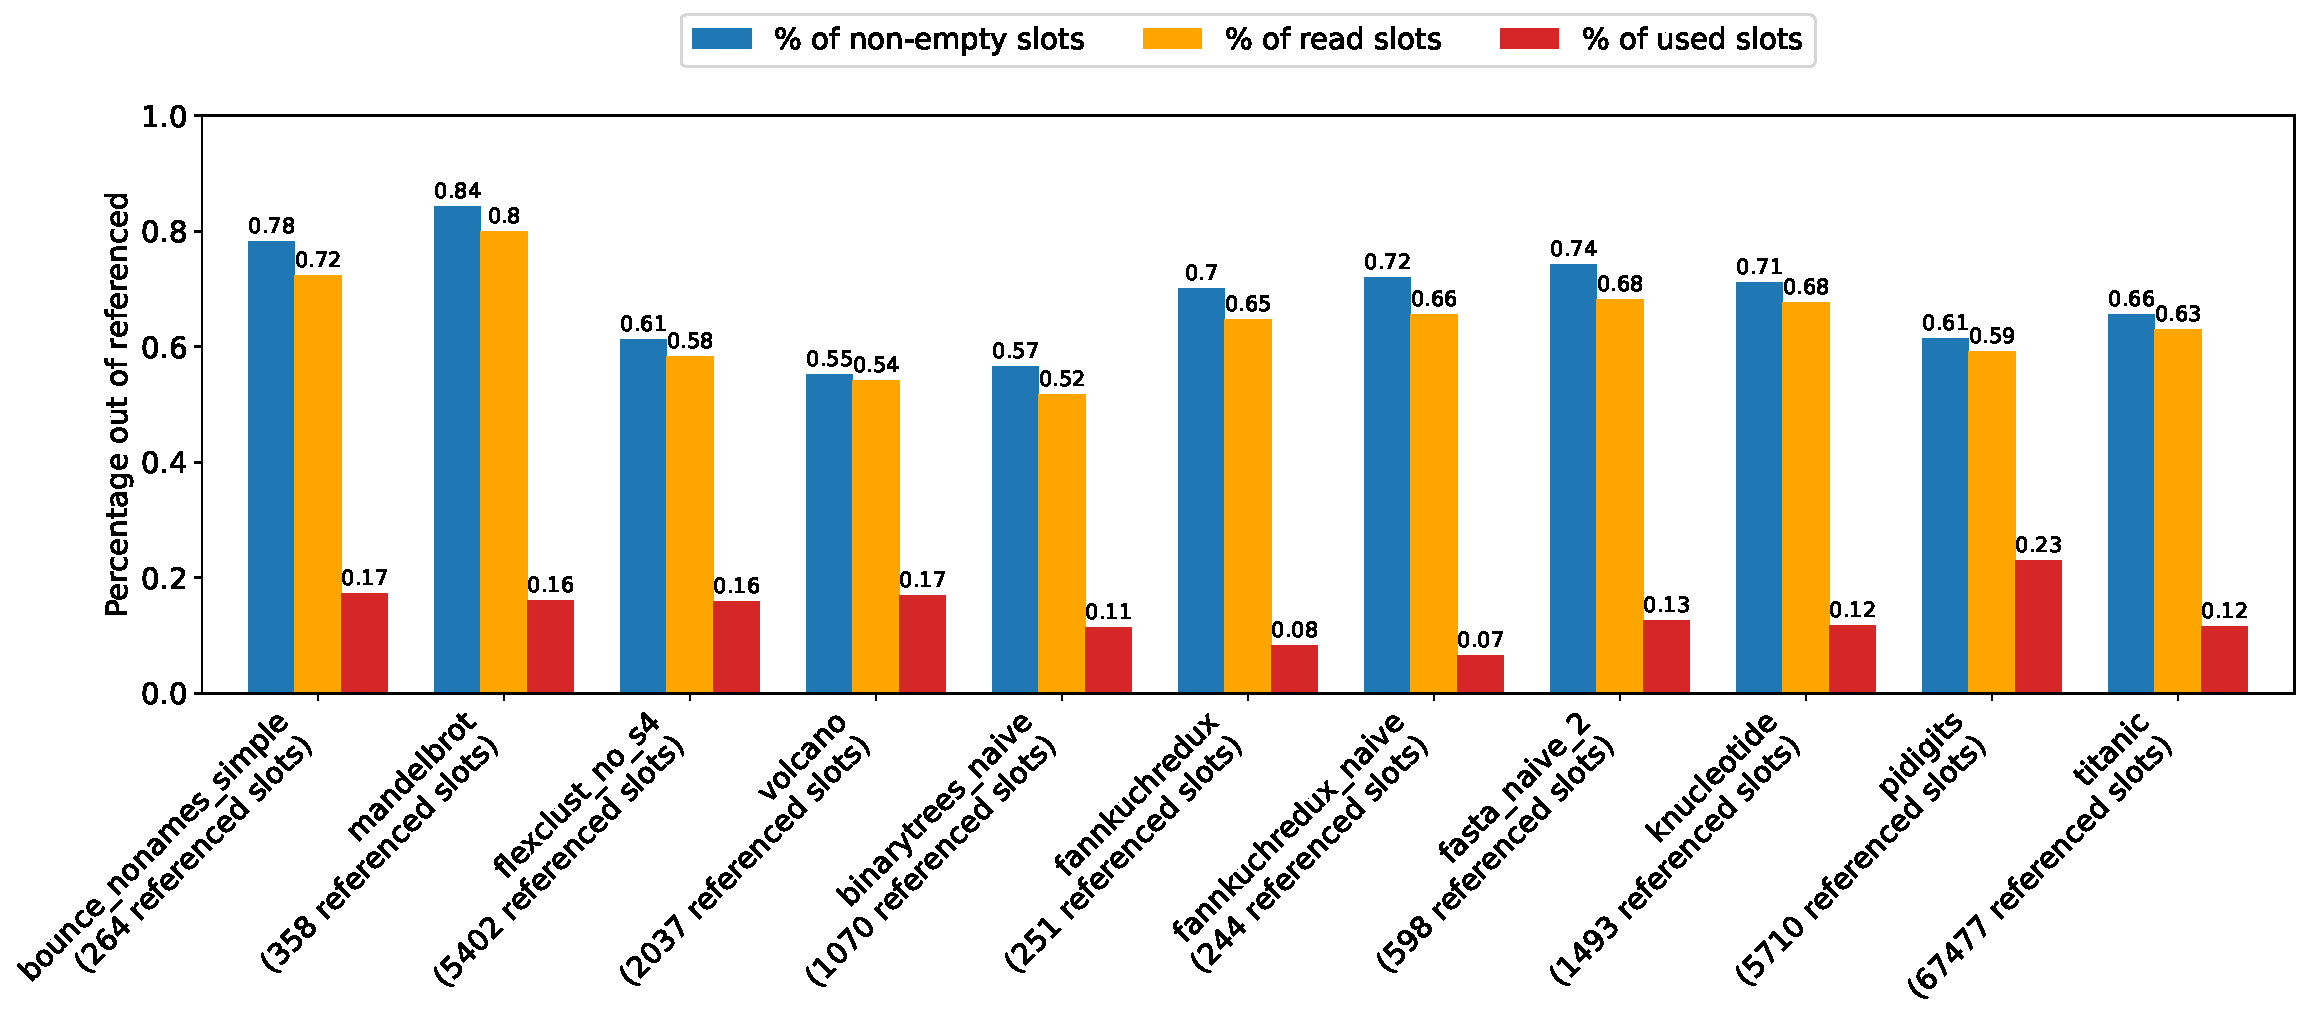
\includegraphics[width=1.5\textwidth]{figures/usage_overall.pdf}
	\end{adjustwidth}
	\caption{Usage of slots across closure compilations}\label{fig:graph-overview}
\end{figure}

When we consider the unused slots shown in figure \ref{fig:graph-unused}, we can see that the dominating cause for a slot not being used is redundancy. This is to be expected in the benchmarks, because they usually only use one numeric type across the whole program. But the Kaggle script uses  a lot of different types, yet 58\% of the unused slots are deemed redundant \todo{why}.

From the slots that are optimized away, on average 62\% of them are also redundant. This suggests to a strong correlation between these categories. 25\% of all slots are neither a redundant, not are they optimized away. This might include some actually redundant slots that are not catched by our aproximate analysis, but there might be also other reasons for not using a slot, like the information in it being too general. These need further analysis.

\begin{figure}
	\centering
	\begin{adjustwidth}{-3cm}{-3cm}
		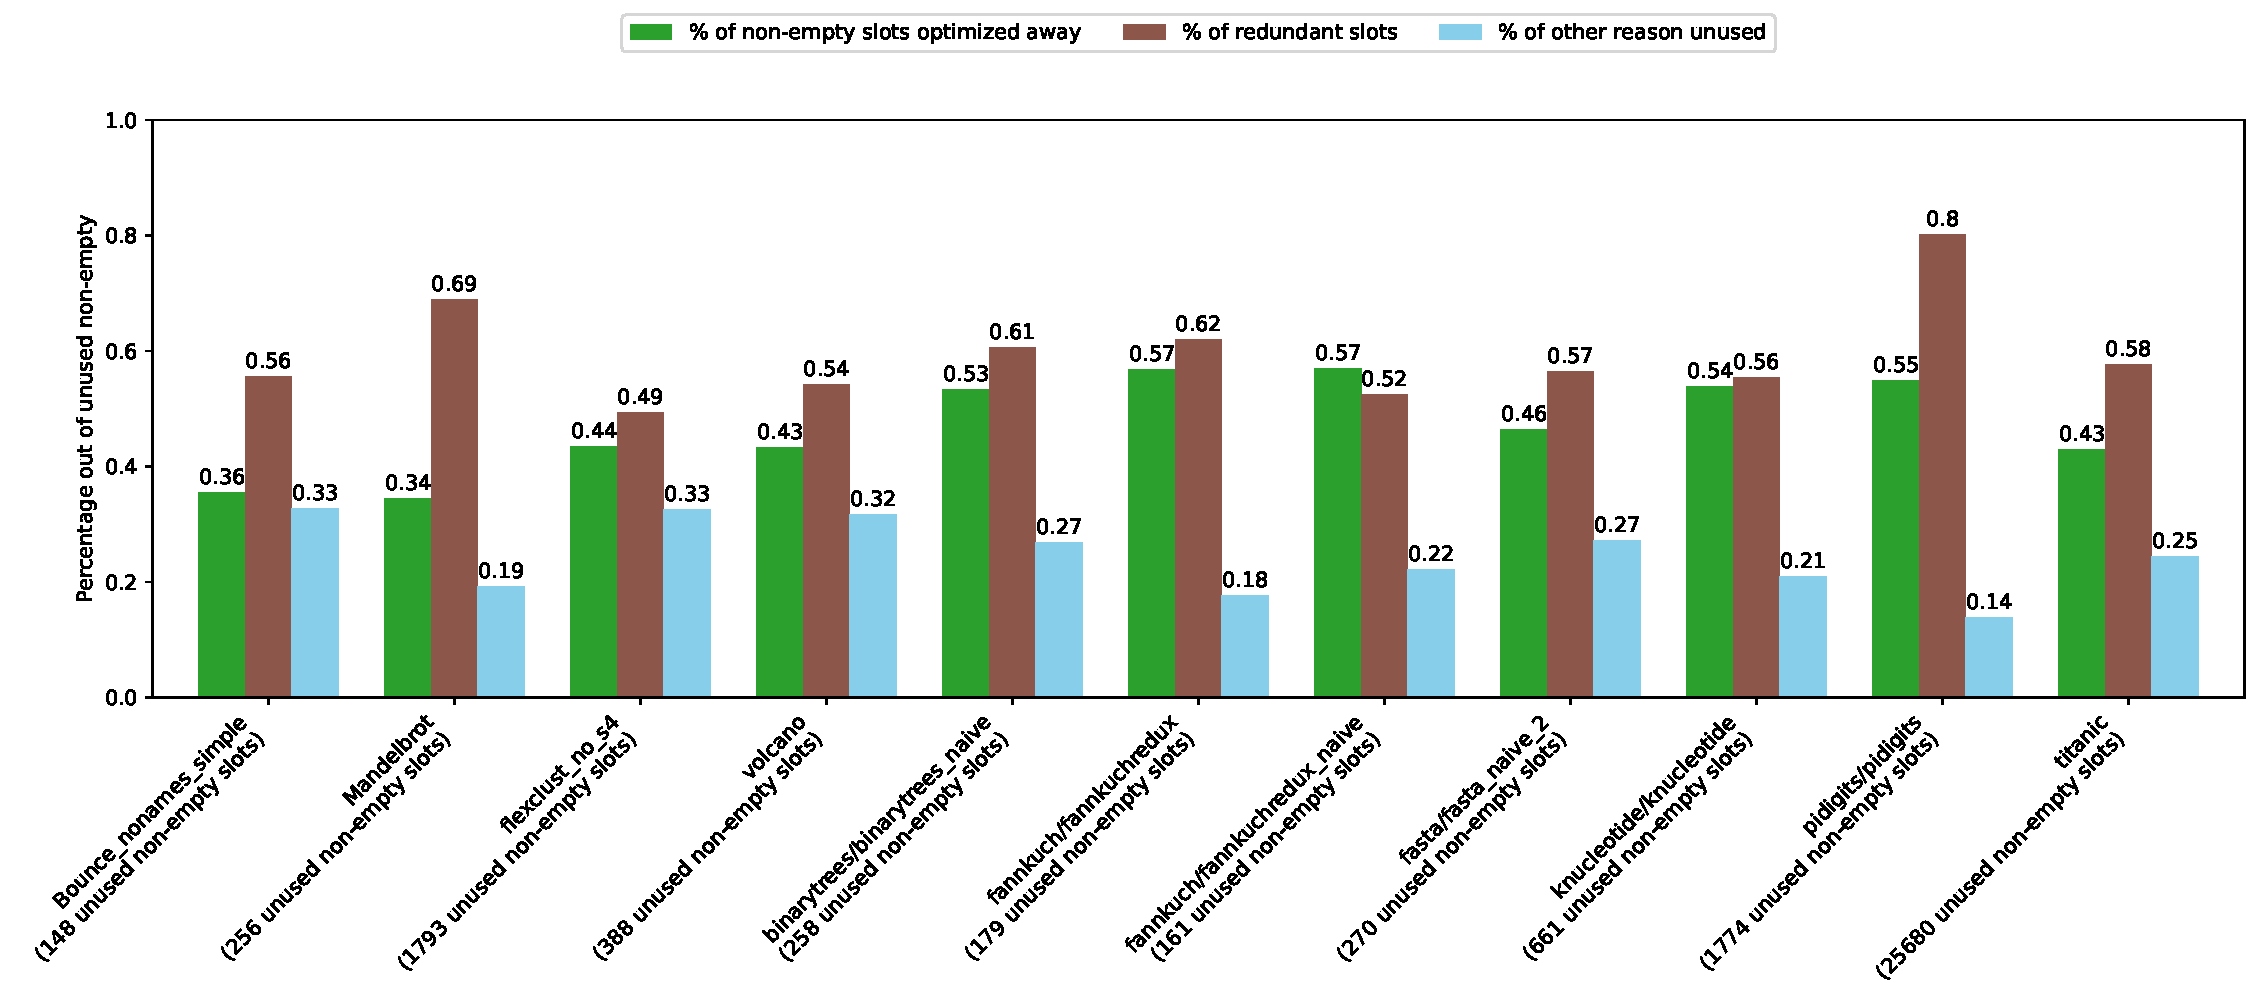
\includegraphics[width=1.5\textwidth]{figures/unused.pdf}
	\end{adjustwidth}
	\caption{Categorization of unused slots across closure compilations}\label{fig:graph-unused}
\end{figure}

When we look on the graph \ref{fig:graph-used}, we can see that more than half of the slots are used as exact match. If we split the monomorphic and polymorphic used slots, we can see an even bigger distinction. On average 81\% of used monomorphic slots are used as exact match. This means that most of the time, when a slot is not polymorphic, it contains an information precise enough to be used as it is. On the other hand, 93\% of used polymorphic slots are widened. This is to be expected, as the polymorphic slots have usually a more general type that does not pass the check for a slot to be used as it is.

For the polymorphic slots used as exact match, the feedback type is either a single non-scalar R type (integer, real or logical), or any R type which might be missing. In either case, the type is always not scalar, but we have observed either that it either has no attributes, or it is not an object. The polymorphism in these cases come from observing both scalar and non-scalar types, or from first observing a type without attributes and subsequently observing a non-object type with attrubutes.

Interestingly, there are very few slots that are narrowed by the static information, 18 to be precise:

\begin{itemize}
	\item{} 2 of them have added information about the type not being NA. Since we do not record this information\footnote{In order to observe that a vector is not NA, we would need to inspect all elements of it and this can be very costly for large vectors}, it is trivial for the static type to narrow it in this way. These are the only monomorphic slots that are narrowed.
	\item{} 4 slots are narrowed into a scalar type. This is due to the slot observing also non-scalar types, but the static type can make this precise.
	\item{} 2 slots have their type narrowed to a double and the only information used from the slot is that the value does not have attributes.
	\item{} In 9 cases, the static type removes a \enquote{might be missing} attribute from the feedback type. In these cases we have observed too many values and the type feedback falls back to the most generic type, which has the attribute that it might be a missing value. But this speculation is on a \texttt{Force} instruction, which when forcing a value that is missing result in an error, thus the result of \texttt{Force} is always not missing or it diverges.
	      \todo{explain missing values?}
\end{itemize}

\todo{For the used slots - only show the avergaes per al/monomorphic/polymorphic}

\begin{figure}
	\centering
	\begin{adjustwidth}{-3cm}{-3cm}
		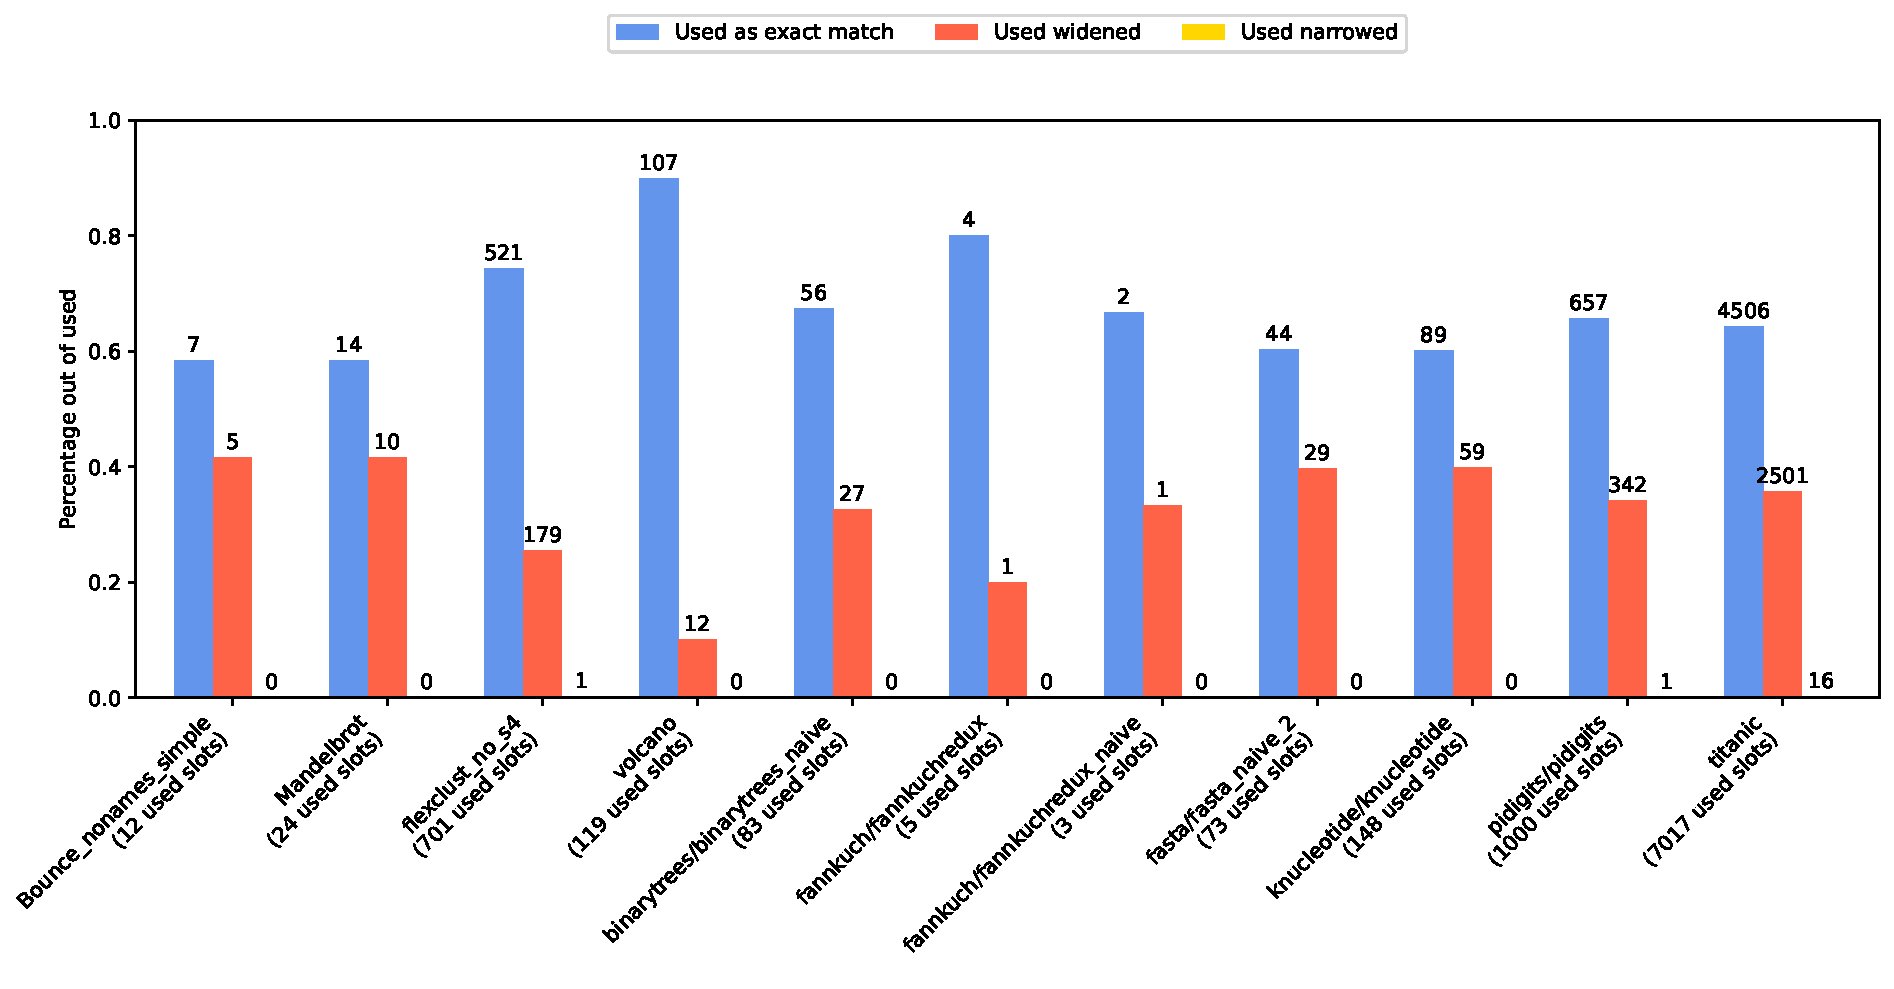
\includegraphics[width=1.5\textwidth]{figures/used.pdf}
	\end{adjustwidth}
	\caption{Categorization of used slots across closure compilations}\label{fig:graph-used}
\end{figure}

\begin{figure}
	\centering
	\begin{adjustwidth}{-3cm}{-3cm}
		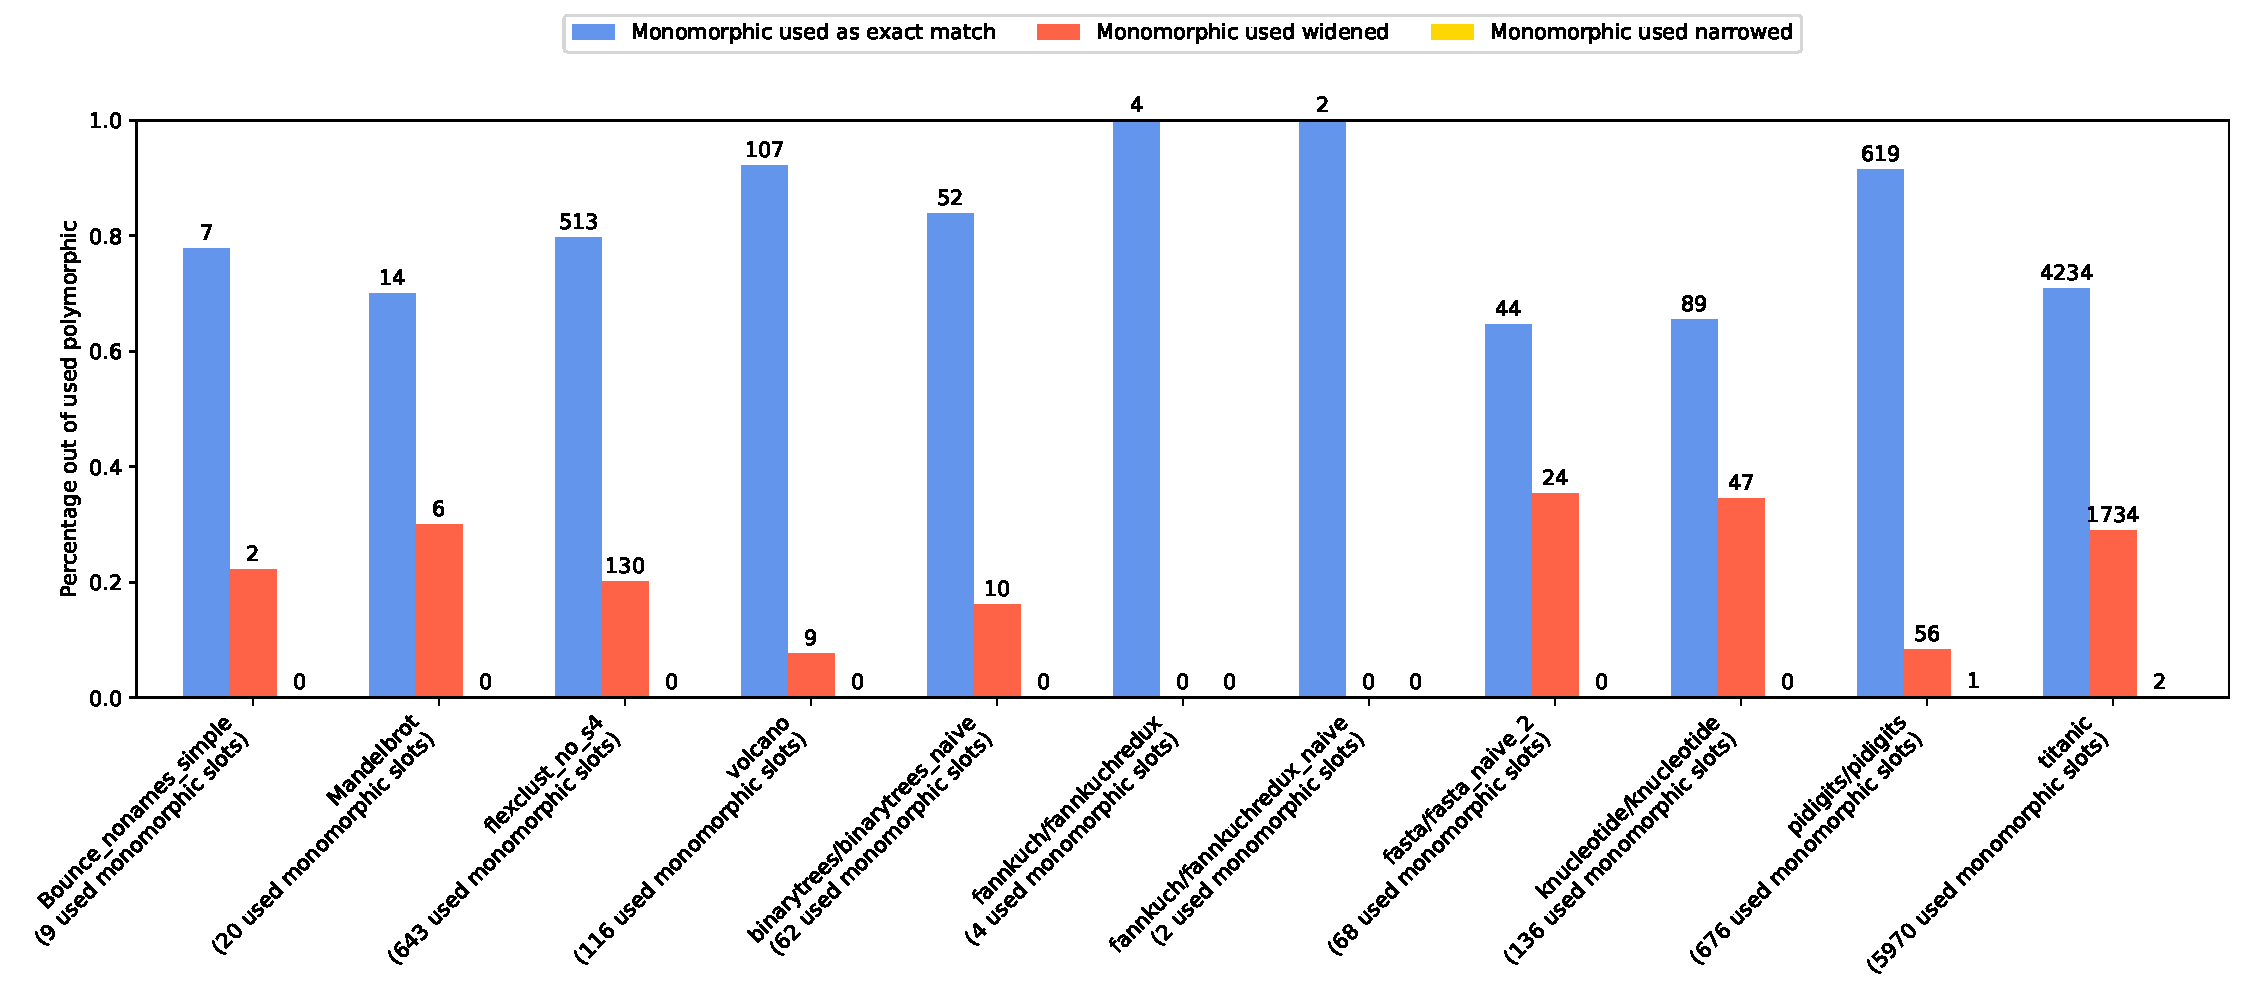
\includegraphics[width=1.5\textwidth]{figures/used_mono.pdf}
	\end{adjustwidth}
	\caption{Categorization of monomorphic used slots across closure compilations}\label{fig:graph-used-mono}
\end{figure}

\begin{figure}
	\centering
	\begin{adjustwidth}{-3cm}{-3cm}
		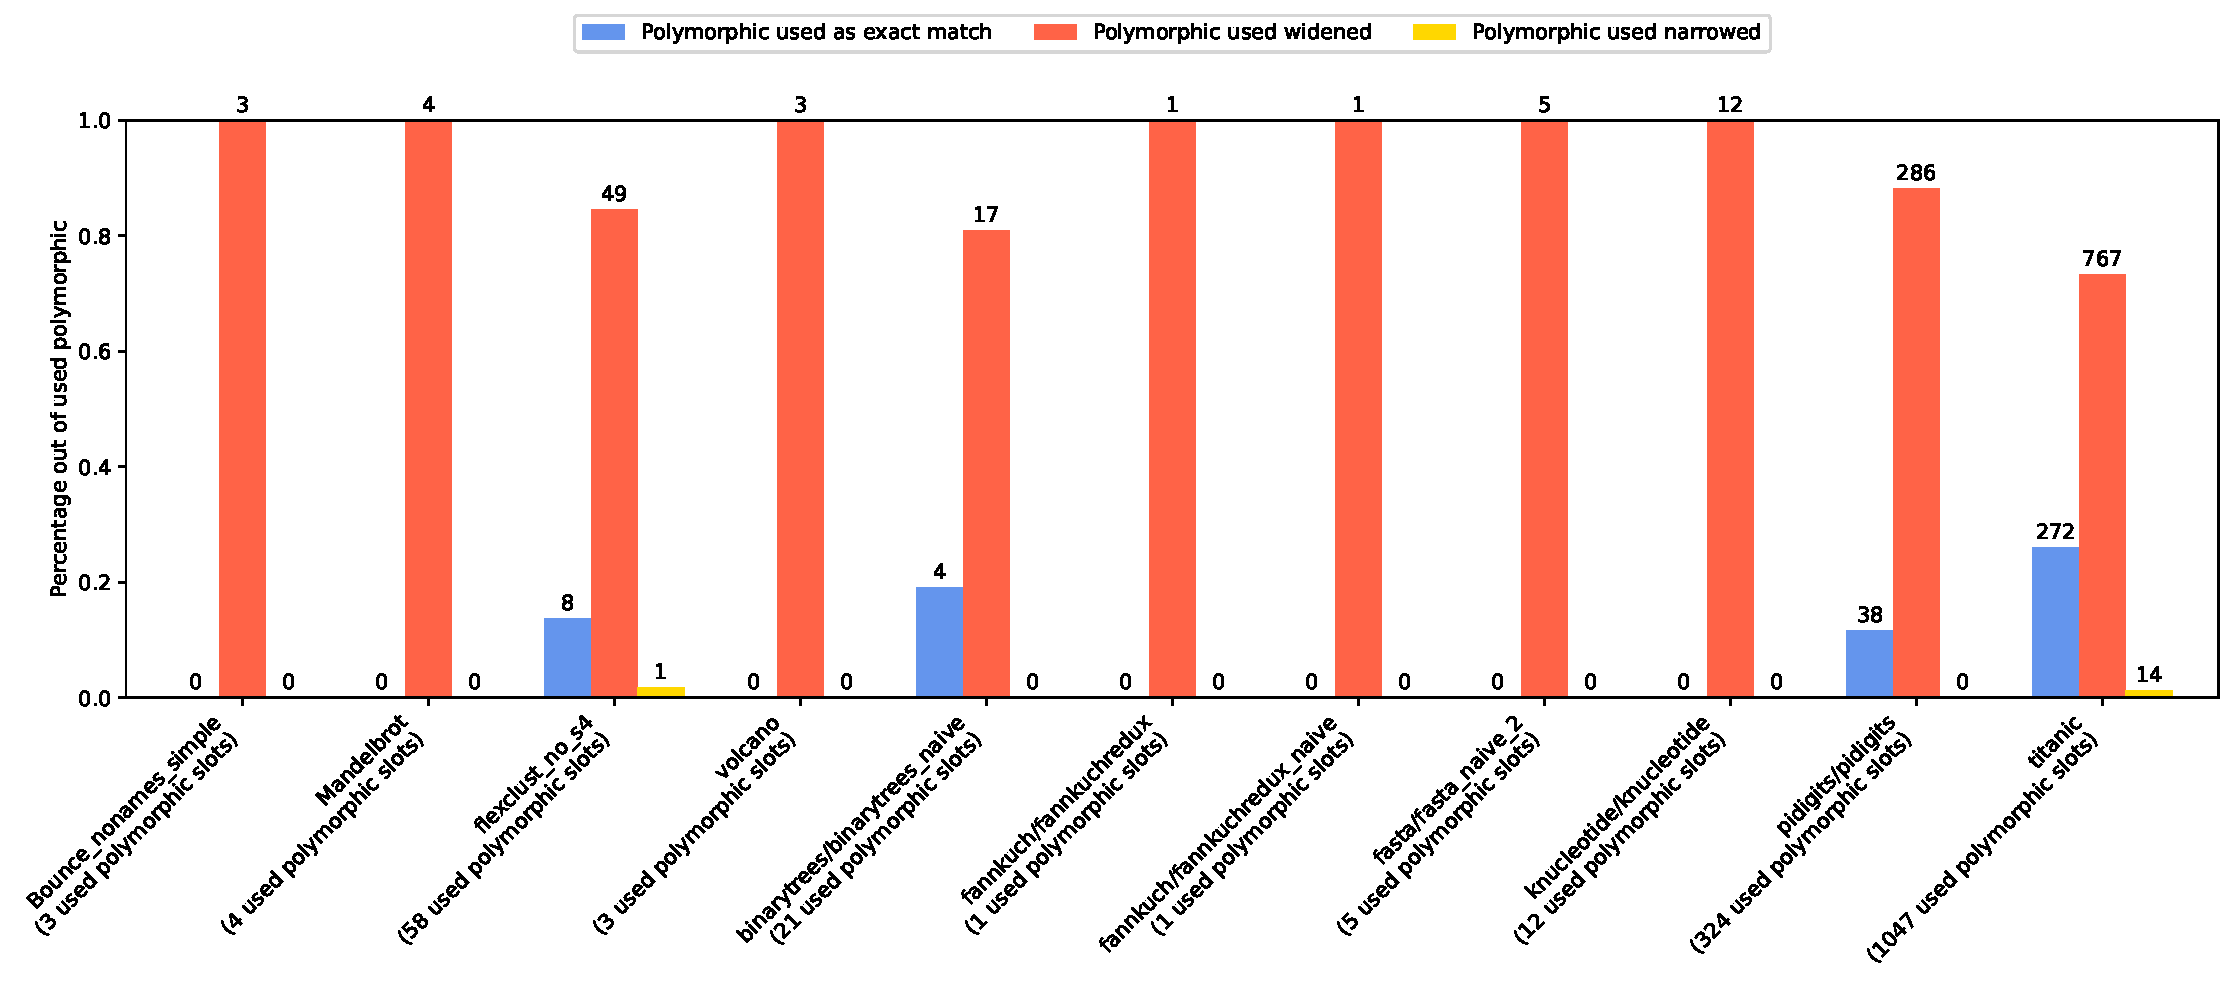
\includegraphics[width=1.5\textwidth]{figures/used_poly.pdf}
	\end{adjustwidth}
	\caption{Categorization of polymorphic used slots across closure compilations}\label{fig:graph-used-poly}
\end{figure}

Unused does not imply polymorphic with probability

used polluted / polluted

polymorphic type => widened

static type - context, bultinins, previous assumes \\
Unable to know how the static type is constructed

An interesting observation is that the Kaggle script behaves very similarly when compared to the benchmarks, only on a different scale. We had a hypothesis that the distribution of slots would be different, because the benchmarks are mostly stable numeric operation written in pure R, whereas the Kaggle script is using a lot of libraries, lots of them having the implementation in C.

%---------------------------------------------------------------
\section{Limitations}
%---------------------------------------------------------------

The biggest drawback of the analysis is the analysis of inlined funcitons. It is not uncommon that a funciton is inlined more than once in a single closure compilation, and this proves to be difficult, as one slot might be used differently. At the same time, inlining a small function many times is going to skew the numbers of the used slots. In our experiments, we observed \todo{how many} slots that were used differently in multiple places, thus we chose to ignore these duplications.

\todo{redundant}
The definition of a redundant slot is very broad and might catch some slots that are not dependent, while at the same time not catch slots that are dependent, but capture a different type. Lets take an example function \texttt{function(x) x + 42}. This function has two type slots, one for the loading of argument \texttt{x} and the second is for the result of \texttt{+}. If we call this funciton with an integer, we record two different types, integer scalar in the first and a double scalar in the second (integer gets coerced into a double). Our analysis will not report any dependency, but from the argument types we truly know the result type. This would require a much more advanced instrumentation of the compiler and might be even

quantifying speed is a very hard problem
nuance of interplay between

%---------------------------------------------------------------
\section{Next steps}
%---------------------------------------------------------------

Reducing recording

Reducing pollution

Relaxing assumptions and ctx

%---------------------------------------------------------------
\subsubsection*{Relaxing assumptions}
%---------------------------------------------------------------

Let's take the example in the listing \ref{lst:assume-example}. This is a function that takes a global variable and when it is a vector of length 1, it returns 33.

When we call it at least once and compile it to PIR, it results in the code \todoadd (omiting deoptimization branches). We can see that the function is pretty optimized. First we load the \texttt{length} function and assume that it is the builtin \texttt{length} (line 8). Then we load the global variablem, force it, and we assume on its type being \texttt{int\$-}, a scalar integer with no attributes (lines 10 and 11). Since we then know it is a scalar, we do not need to call the builtin length function and this allows us to constant fold the if statement, thus we return the number 33.

The problem is when we reassign the variable \texttt{G} to a different scalar like \texttt{G <- 42}. The code is still valid, as the only part of the information that is used is the scalar. Event thought we only need to assume on \textit{is scalar} part, we assume on something more specific (is a scalar integer and has no attributes). Thus, when we call the function again after reassigning G to a double \texttt{42}, we trigger a deopt.

\begin{listing}
	\begin{minted}{R}
G <- 42L

f <- function() {
  if (length(G) == 1){
    33
  }
}
  \end{minted}
	\caption{Example of wide type assumtion}\label{lst:assume-example}
\end{listing}

\begin{listing}
	\begin{minted}{\pirlexer}
BB0
  goto BB1
BB1   <- [0]
  %1.0  = LdVar              length, R_GlobalEnv
  %1.1  = Identical          <blt length>, %1.0   <true>
  %1.2  = Checkpoint          -> BB2 (default) | BB3 (if assume failed)
BB2   <- [1]
          Assume             %1.1, %1.2 (DeadBranchReached[Test#0])
  %2.1  = LdVar              G, R_GlobalEnv
  %2.2  = IsType             %2.1 isA int$-
          Assume             %2.2, %1.2 (Typecheck[Type#1])
          Visible
          Return             33
  \end{minted}
	\caption{PIR code generated for listing \ref{lst:assume-example}, omiting deopt branches}\label{lst:assume-example-pir}
\end{listing}

